% Szglab4
% ===========================================================================
%
\chapter{Követelmény, projekt, funkcionalitás}

\thispagestyle{fancy}

\section{Bevezetés}

\subsection{Cél}

A project követelményeinek, alapvető felépítésének és funkcionalitásának ismertetése, ezek segítségével a fejlesztési folyamatok majd a végleges program felépítésének megtervezése. Fejlesztés közben ezeket figyelembe kell majd venni és tőlük eltérni nem szabad.

\subsection{Szakterület}
A project a Szoftver laboratórium 4. tantárgy feladatának megoldására született. Az elkészítendő szoftver egy számítógépes játék, nem kimondottan egy szakterület részére készül, inkább szórakoztatás céljából.

\subsection{Definíciók, rövidítések}
\begin{itemize}
\item \textbf{BME}	Budapesti Műszaki Egyetem rövidítése.
\item \textbf{Doxygen}	Forráskódból és kommentekből dokumentációt generáló program.
\item \textbf{Eclipse}	Fejlesztőkörnyezet Java programozási nyelvhez.
\item \textbf{Git}	Verziókezelői rendszer.
\item \textbf{Google Calendar}	Google egy szolgáltatása, melyben eseményeket lehet beállítani naptárszerűen. Ezek megoszthatók más felhasználókkal is.
\item \textbf{Google Mail}	Google egy szolgáltatása, mely az internetes levelezést biztosítja a felhasználóinak.
\item \textbf{HSZK}		Hallgatói Számítógép Központ rövidítése.
\item \textbf{HUD}	Head-Up Display rövidítése. Egy szem elé vetített kijelző, melyen a fontosabb, illetve alapvető adatokat jelenítik meg.
\item \textbf{IDE}	Integrated Development Environment (Integrált Fejlesztői Környezet) rövidítése. A számítógép programozást megkönnyítő programok ezek.
\item \textbf{IntelliJ}	Java IDE, megkönnyíti a fejlesztést.
\item \textbf{JDK}	Java Development Kit (Java Fejlesztői Készlet) rövidítése. A Java nyelv fejlesztőeszköze.
\item \textbf{JRE}	Java Runtime Environment rövidítése. Program, ami szükséges a Javában megírt fájlok elkészítéséhez, futtatásához.
\item \textbf{LaTex}		Dokumentum formázó rendszer, mellyel magas színvonalú dokumentációk készíthetők.
\item \textbf{Netbeans}	Fejlesztőkörnyezet, ami Java nyelven alapul. A programban egyszerűen, gyorsan lehet grafikus felületet létrehozni, például menüket.
\item \textbf{PC}	Personal Computer rövidítése. Jelentése: személyi számítógép, manapság a legtöbb számítógép ilyen.
\item \textbf{prototípus}	A program azon állapota, melyben meg van valósítva minden funkció működőképesen, de a grafikus felület még nincs beleépítve.
\item \textbf{ShareLaTeX}	Internetes LaTeX szerkesztő, mely lehetővé teszi dokumentumok szerkesztését, előkészítését valós idejű online környezetben.
\item \textbf{Sympa}	Egy szoftver, mely lehetővé teszi a levelező listák használatát, menedzselését.
\item \textbf{szkeleton}	A program azon állapota, melyben a belső felépítés készen van (a függvények osztályok), de még nem csinál semmit.
\item \textbf{szoftver}	A számítógépen elhelyezhető, futtatható program.
\item \textbf{use-case}	Lehetséges interakciók leírása a rendszer és az aktor (felhasználó) között.
\item \textbf{verziókezelés}		Olyan tevékenység, amellyel eltárolhatóak a fájlok régebbi verzió, ezáltal egy-egy módosítás után vissza lehet térni egy adott verzióhoz és nyomon lehet követni a fejlesztést.

\end{itemize}

\subsection {Hivatkozások}
Szoftver Labor 4 - \url{https://www.iit.bme.hu/~szoftlab4/}

GitHub - \url{https://github.com/tht-krisztian/Szoftlab4.git}

\subsection{Összefoglalás}
A dokumentum további részeiben található:
\begin{itemize}
\item 2.2 Áttekintés: A project terveinek, funkcióinak áttekintése, a felhasználók lehetőségeinek áttekintése
\item 2.3 Követelmények: A project során elvárt követelmények kidolgozása, külön kitérve funkcionális, erőforrás, átadással kapcsolatos és egyéb nem funkcionális követelményekre.
\item 2.4 Lényeges use-case-ek felsorolása, use-case diagram
\item 2.5 Szótár: A project során bevezetett fogalmak körülírása.
\item 2.6 Project terv: A project résztvevőinek feladatkörei és határidők részletes kifejtése
\item 2.7 Napló: Az elvégzett feladatok és ráfordított idő felsorolása
\end{itemize}
\pagebreak

\section{Áttekintés}
\subsection{Általános áttekintés}


\begin{figure}
\centering
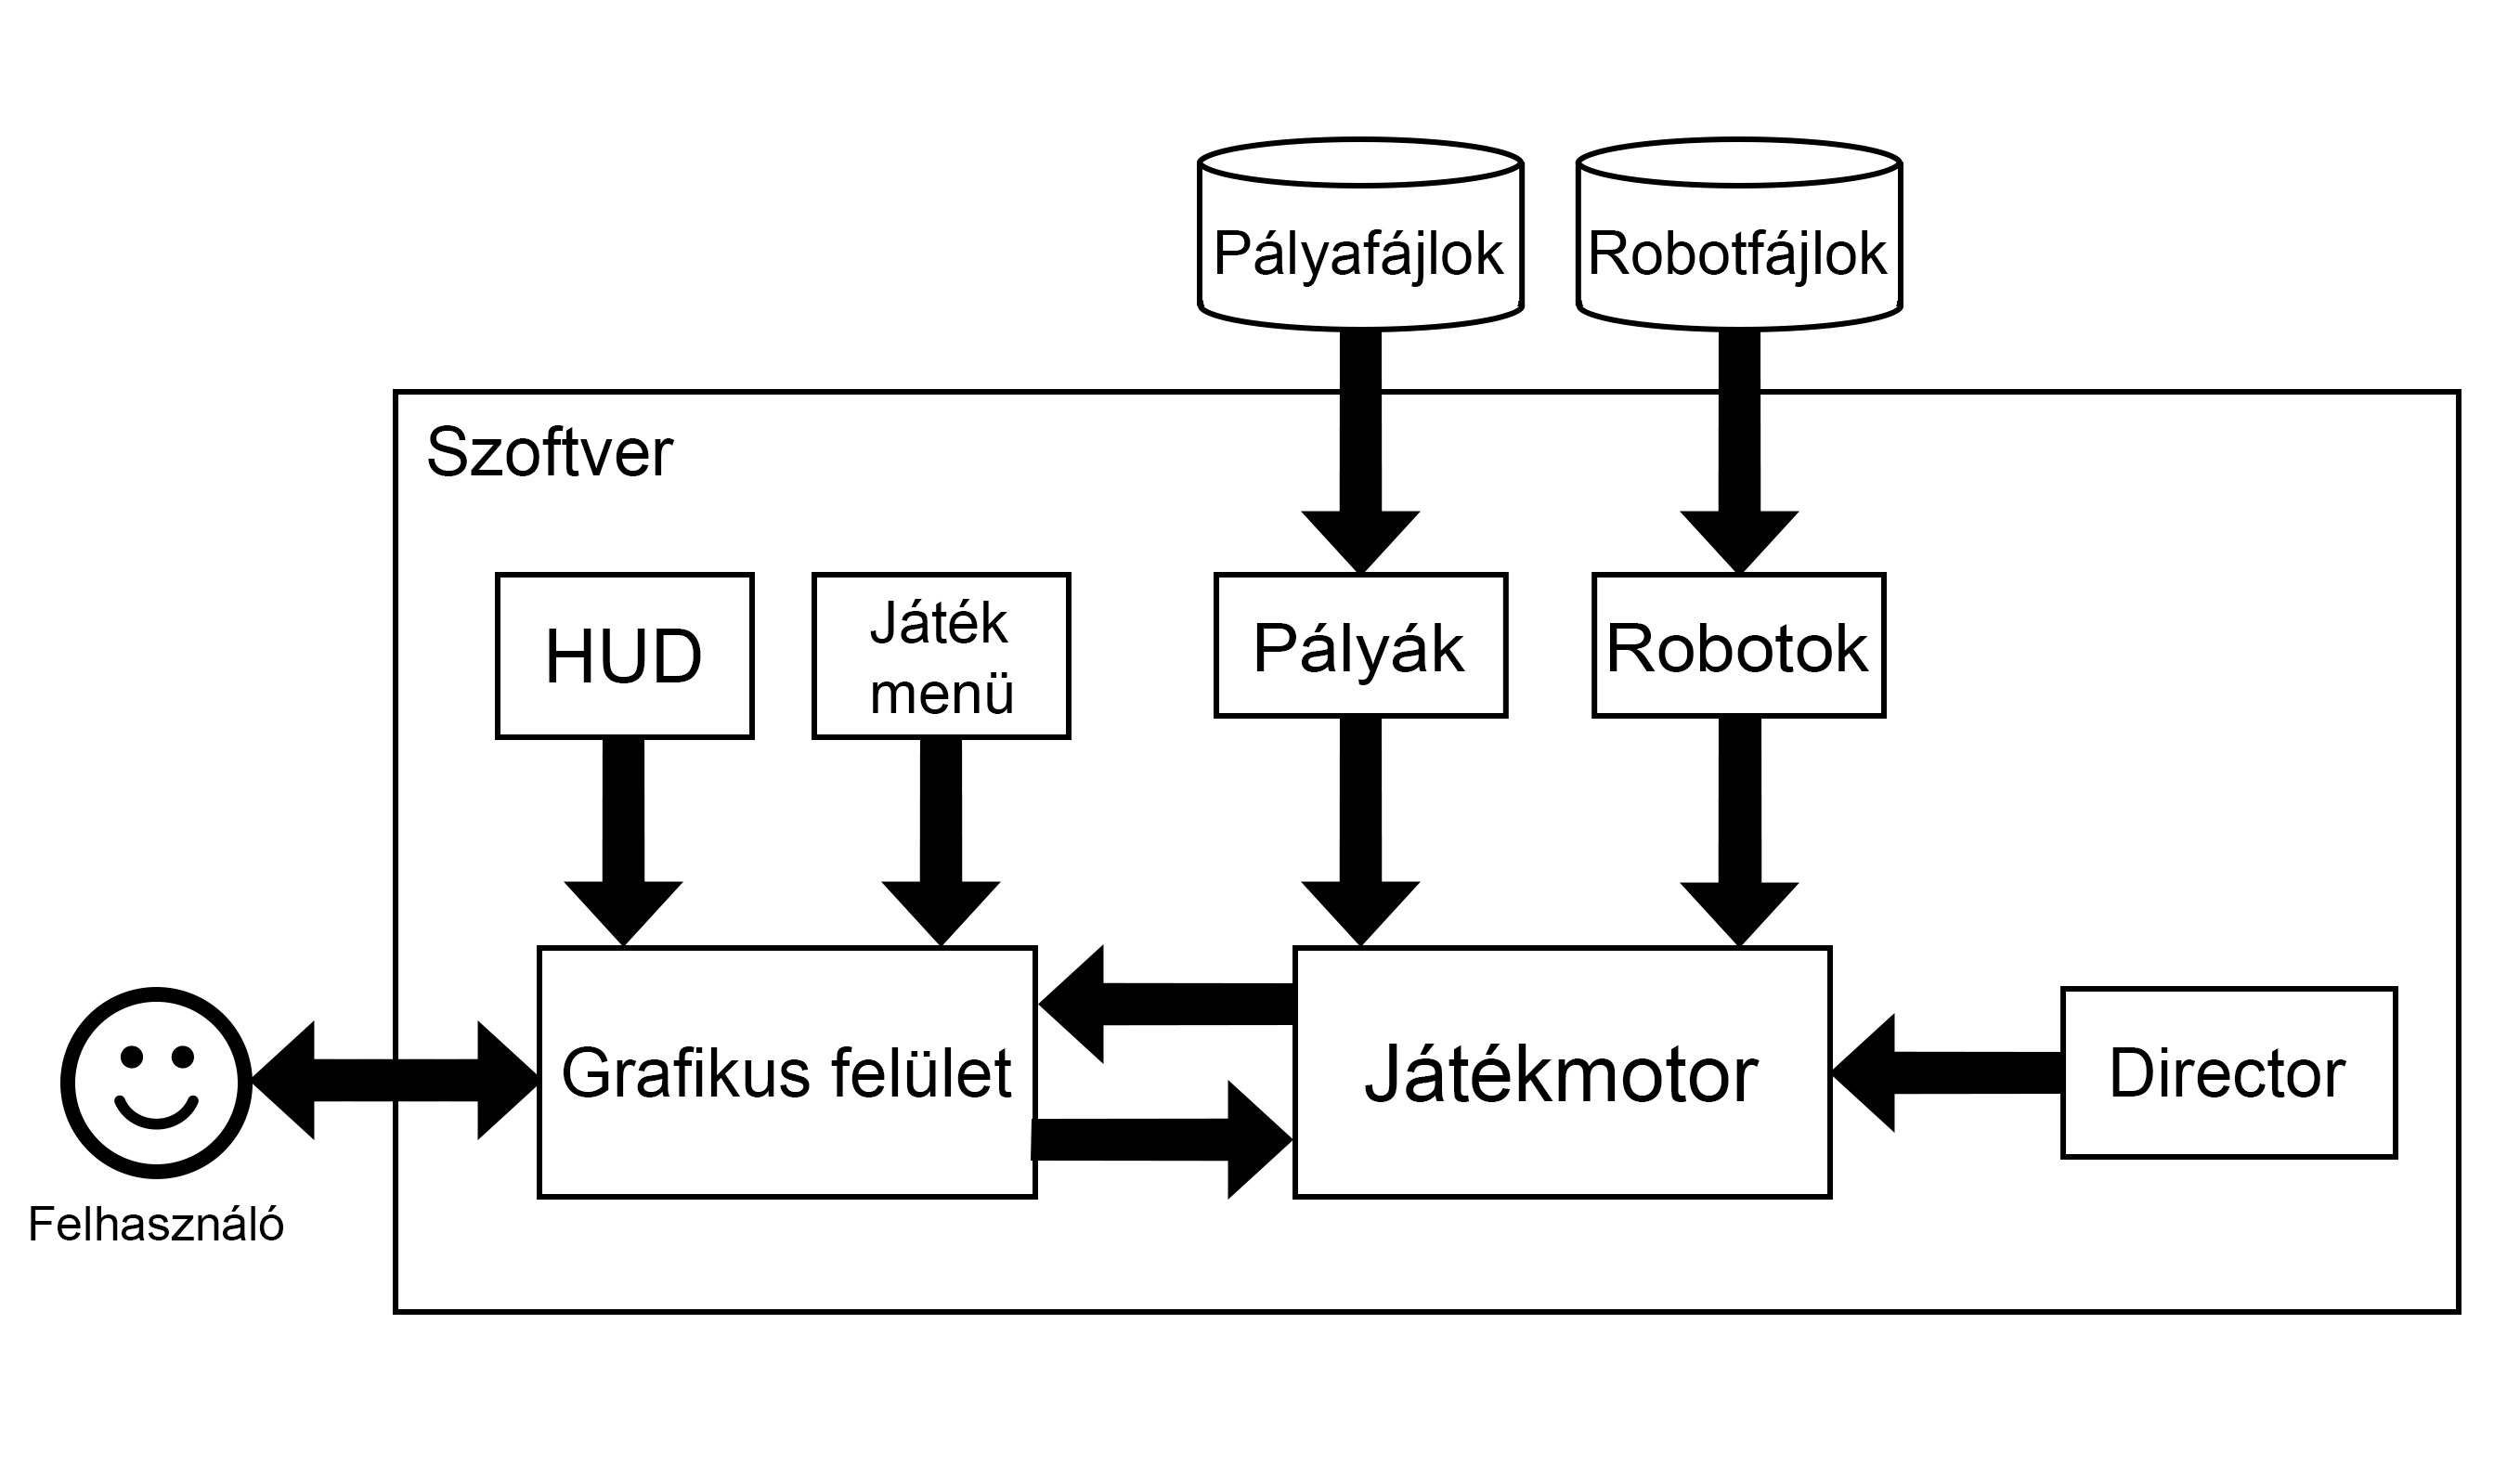
\includegraphics[scale=0.17]{arch_kep.jpg}
\caption{Architekturális kép}
\label{fig:my_label}
\end{figure}

A szoftver fontos eleme a Játékmotor. Ez teremti meg a kezdeti feltételeket és irányítja a játék folyását. Ez fogja ellenőrizni, hogy a robotok leesnek-e a pályáról, ha olajfoltba lépnek letiltja az irányítást a játékos oldalon, illetve ha ragacsba lép egy játékos, akkor lelassuljon. A Játékmotor indulása előtt lekéri a Pályák alrendszertől a kiválasztott pályát.

A director alrendszer feladata az idő léptetése,  a robotok másodpercenkénti ugrását ütemezi.

A HUD alrendszer hivatott jelezni, hogy a játékos számára elérhető-e az olaj vagy ragacskészlet, továbbá a megtett körök számát.

A játék menü alrendszer feladata a játék során a megfelelő parancsra megállítani a játékot és a beállítások (pl.: grafikai, hang) állíthatósága.

A grafikus felület feladata, hogy kapcsolatot létesítsen a játékossal vizuális információkkal és a játékos ezen keresztül irányíthatja a játékmotort. Továbbá hozzáfér a játék menühöz és a HUD-hoz, hiszen ki kell jeleznie azokat.

A Pályák alrendszer betölti a Pályafájlokból a pályákat, tárolja, majd azokat a Játékmotor rendelkezésére bocsájtja.

A Robotok alrendszer betölti a robotokat a Robotfájlokból, tárolja azokat, majd a Játékmotor rendelkezésére bocsájtja.

Hálózatot a szoftver nem igényel. Háttértáron pedig a program .jar archívumainak, a kirajzoláshoz szükséges pálya és robot képeknek, a pályákat tartalmazó fájloknak szükséges helyet biztosítani. Ezeken kívül nincs szükség futás idejű tárhelyigényre. 

\subsection{Funkciók}
Mivel unalmas a mérnökök munkája a Marson (nem adnak nekik elég érdekes feladatot, mint például a napelem-építés, vagy az ásványi anyag gyűjtése), ezért robotokat versenyeztetnek egymás ellen; ezt valósítja meg az alábbi játékprogram.

Egy versenyző játéknak a lényege, hogy a résztvevők egymás ellen próbálnak minél tovább eljutni a pályán, illetve minél jobb időt elérni. Ez itt sincs másként, a verseny célja, hogy a megadott idő alatt több kört tegyünk meg robotunkkal mint az ellenfél. Ebben segítségünkre lehet a pálya kialakítása, és a különböző felszerelések, melyek megnehezíthetik a verseny lefutását. Fontos, hogy a robotok a kijelölt pályán maradjanak, mert csak ezen a területen biztosított a kommunikáció a vezérlőközponttal. Ha egy robot elhagyja a pályát diszkvalifikálják a futamból.

Az idő lejártával (esetleg más játékmódoknál egy adott körszám megtétele után) a játék véget ér. Ebben az esetben az a játékos robotja nyer, amelyik több kört tett meg (vagy elsőként ért be a célba adott kör után), kivéve ha idő előtt letér a pályáról, ezáltal nem vesz részt az eredményhirdetésen a célvonalnál.

A játékteret a csodálatos Mars környezete adja, ami nagyon veszélyes terep. Tartani kell a különféle sugárzásoktól, nehogy kárt tegyenek a mérnökökben és a nézőkben, ezért ők egy védett szobából szemlélik és irányítják az eseményeket. A pályán különféle nehezítések is helyet kapnak, hogy ne legyen a robotoknak (és mérnökeiknek) könnyű az élete. Olyan akadályokkal kell megbirkózniuk a robotoknak, mint például a lyukak elkerülése, melyek a felépítésüket teszik tönkre, ezáltal nem tudnak tovább versenyezni, vagy az olajfoltok időben való észrevétele, ami meggátolja, hogy a mérnökök irányítsák őket, végül de nem utolsó sorban a ragacsokat is ki kell kerülniük, mert azok a sebességüket csökkentik, ezáltal nagy előnyt adva az ellenfél robotjának. A többi robothoz sem éri meg közel tartózkodni, hiszen mint minden verseny alatt, az ütközésnek itt is ára van, ez most az irányítás bezavarodásában merül ki. Végül a legnagyobb akadály maga a pálya. A versenyeket egy lapos fennsíkon szokták tartani a Marson, jól elszeparálva a marslakóktól, hogy azok ne tudjanak belekontárkodni a futamba, de elakadhatnak vagy leeshetnek a szélén, a mérnököknek erre is nagyon kell figyelniük az irányítás alatt.

A robotok a startvonalról indulnak úgy, hogy figyelembe véve a pálya felépítését, igazságos legyen minden résztvevőnek (a mérnökök a pályán kívülről irányítják őket). A „Start”-ot egy visszaszámolás indítja, melynek következtében a robotok elindulnak. A pályán állomások találhatók, melyek minden robot áthaladásánál ellenőrzik, hogy nem történt-e csalás. Minden körben a pályán adott állomásokon kell áthaladni adott sorrendben. A kör csak akkor érvényes, ha a robot ezeknek a megszorításoknak eleget tud tenni. Továbbá a távolság mérése (ezáltal győzelmi feltételek) is ez alapján történik, szóval egyik mérnöknek sem éri meg ide-oda navigálni a robotját a pontok között, a legnagyobb megtett út reményében.
A robotok sebessége állandó, a mérnökök csak az ugrások irányát tudják befolyásolni a játék lezajlása alatt, ezért nagyon kell figyelni, hogy a kanyarokat jó ívben vegyék be, az akadályokat pedig megfelelő szakértelemmel kerüljék ki. Továbbá az indulás után máris lehetőséget nyújt a játék, hogy a mérnökök használják a robotokba beépített felszereléseket. Ezek nem mások mint a már feljebb leírt ragacsok és olajfoltok. Ezeket maguk mögött képesek hagyni, és a játék végéig megmaradnak a pálya felületén (illetve amíg valaki bele nem megy, akár a mérnök saját robotja), fejfájást okozva ezzel a versenyzőknek. A felszerelések körönként (fentebb említett „Checkpoint-rendszer” szerint) újratöltődnek, ezért a mérnököknek nem kell taktikázniuk, hogy mikor törjenek borsot az ellenfelük orra alá; körönként megtehetik azt.

A verseny ezen lehetőségek megvalósítása által igen érdekes, veszélyes és néha akár frusztráló is, gondoljunk csak a robotok felszereléseire. Egyszóval ideális időtöltés a Marson unatkozó mérnököknek.

\subsection{Felhasználók}
A játék 2 játékos módban indíthat. A játékosnak semmiféle előképzettségre nincs szüksége, a játék menete gyorsan elsajátítható. A játékban nem lesz pályaszerkesztő. A játékot nem lehet elmenteni, mindig újból kell kezdeni.

\subsection{Korlátozások}
A BME IIT Szoftver Laboratórium tantárgy oktatói (a megrendelők) által kiírt specifikáció megköveteli, hogy a program a HSZK gépein a beadások alkalmával futtathatók legyenek. Ezekre a gépekre már előre feltelepített JRE 1.7-es környezet elérhető, ezért csak a JDK 1.6-es verziójaban már létező függvények, osztályok használhatóak a kód megírása során.


\subsection{Feltételezések, kapcsolatok}
\textbf{Szoftver Labor 4}
\begin{itemize}
\item feladat határidői \url{https://www.iit.bme.hu/~szoftlab4/}
\item feladatkiírás \url{https://www.iit.bme.hu/~szoftlab4/feladat.shtml}
\item dokumentáció sablonok \url{https://www.iit.bme.hu/~szoftlab4/templ/}
\end{itemize}

 

\section{Követelmények}
\subsection{Funkcionális követelmények}

% Azonosító, Leírás, Ellenőrzés, Prioritás, Forrás, Use-case, Komment
\begin{longtable}{| l | l | l | l | l | l | l |}
\hline
\textbf{Azonosító}   & \textbf{Leírás} & \textbf{Ellenőrzés} & \textbf{Prioritás} & \textbf{Forrás} & \textbf{Use-case} & \textbf{Komment} \tabularnewline
\hline 1.01 & Játék menü & bemutatás & alapvető & csapat & &\tabularnewline
\hline 1.02 & Beállítások kezelése & bemutatás & opcionális & csapat & &\tabularnewline
\hline 1.03 & Játék elindítása & bemutatás & alapvető & megrednelő &\vtop{\hbox{\strut Új Játék}\hbox{\strut indítás}}&\tabularnewline
\hline 1.04 & Pályáról leesők kiesnek & bemutatás & alapvető & megrendelő & &\tabularnewline
\hline 1.05 & Előre elkészített versenypálya & bemutatás & alapvető & megrendelő & &\tabularnewline
\hline 1.06 & \vtop{\hbox{\strut Robotok a kezdőpozíciójukból}\hbox{\strut indulnak}}& bemutatás & alapvető & megrendelő & &\tabularnewline
\hline 1.07 &\vtop{\hbox{\strut Pályán vannak olajfoltok és}\hbox{\strut ragacsfoltok}}& bemutatás & alapvető & megrendelő & &\tabularnewline
\hline 1.08 &\vtop{\hbox{\strut Robotok fel vannak szerelve }\hbox{\strut olaj és ragacskészlettel}} & bemutatás & alapvető & megrendelő & &\tabularnewline
\hline 1.09 &\vtop{\hbox{\strut 2 személy tudjon játszani}\hbox{\strut egyszerre}} & bemutatás & alapvető & csapat & &\tabularnewline
\hline 1.10 &  Körlimites játékmód & bemutatás & opcionális & csapat & &\tabularnewline
\hline 1.11 &  Időlimites játékmód & bemutatás & alapvető & megrendelő & &\tabularnewline
\hline 1.12 & A robotok tudjanak ugrani & bemutatás & alapvető & megrendelő & &\tabularnewline
\hline 1.13 &\vtop{\hbox{\strut A ragacs és olaj a pályáról}\hbox{\strut idő után eltűnik}} & bemutatás & opcionális & csapat & &\tabularnewline
\hline 1.14 & \vtop{\hbox{\strut A ragacs és olaj a pályáról,}\hbox{\strut ha belelépnek eltűnik}} & bemutatás & opcionális & csapat & &\tabularnewline
\hline 1.15 & \vtop{\hbox{\strut A robotok tudnak egymással}\hbox{\strut ütközni}} & bemutatás & opcionális & csapat & &\tabularnewline
\hline 1.16 &\vtop{\hbox{\strut Az indulás előtt}\hbox{\strut visszaszámlálás indul}} & bemutatás & opcionális & csapat & &\tabularnewline
\hline 1.17 &\vtop{\hbox{\strut A robotok sebessége }\hbox{\strut egységnyi méretű tetszőleges }\hbox{\strut irányú vektorral módosítható }} & bemutatás & alapvető & megrendelő & &\tabularnewline
\hline 1.18 &\vtop{\hbox{\strut Egy ugrással a sebességgel}\hbox{\strut egyenesen arányos}\hbox{\strut{távolságra tudnak eljutni}}} & bemutatás & alapvető & megrendelő & &\tabularnewline
\hline 1.19 &\vtop{\hbox{\strut A robot ragacsra érkezve}\hbox{\strut sebessége a felére csökken}} & bemutatás & alapvető & megrendelő & &\tabularnewline
\hline 1.20 &\vtop{\hbox{\strut A robot olajfoltra érkezve}\hbox{\strut sebességének módosítása}\hbox{nem lehetséges}} & bemutatás & alapvető & megrendelő & & \tabularnewline
\hline 1.21 &\vtop{\hbox{\strut A robot olajat vagy}\hbox{\strut ragacsot tudnak lerakni}} & bemutatás & alapvető & megrendelő & \vtop{\hbox{\strut Akadá-}\hbox{\strut lyozás}} & \tabularnewline
\hline 1.21 & A játékból ki  lehet lépni & bemutatás & alapvető & megrendelő & Kilépés & \tabularnewline

\hline
\end{longtable}

\subsection{Erőforrásokkal kapcsolatos követelmények}

% Azonosító, Leírás, Ellenőrzés, Prioritás, Forrás, Komment
\begin{longtable}{| l | l | l | l | l | l |}
\hline
\textbf{Azonosító}   & \textbf{Leírás} & \textbf{Ellenőrzés} & \textbf{Prioritás} & \textbf{Forrás} & \textbf{Komment} \tabularnewline
\hline
\hline 2.01 & JRE  & bemutatás  & alapvető  & megrendelő & Java IDE  \tabularnewline
\hline 2.02 & Eclipse & nincs & opcionális & csapat & Java IDE \tabularnewline
\hline 2.03 & NetBeans IDE & nincs  & opcionális  & csapat  & Java IDE  \tabularnewline
\hline 2.04 & IntelliJ IDEA & nincs  & opcionális  & csapat  & Java IDE  \tabularnewline
\hline 2.05 & ShareLatex & nincs  & opcionális  & csapat  & online LaTeX editor  \tabularnewline
\hline 2.06 & ShareLatex & nincs  & opcionális  & csapat  & online LaTeX editor  \tabularnewline
\hline 2.06 & Git & nincs  & alapvető  & csapat  & Elosztott verziókezelő \tabularnewline
\hline 2.07 & GitHub account & nincs  & alapvető & csapat & Git tárhely \tabularnewline
\hline 2.08 & PC & bemutatás  & alapvető  & megrendelő  &  \tabularnewline
\hline 2.09 & Monitor & nincs  & alapvető  & csapat  &  \tabularnewline
\hline 2.10 & Billentyűzet & nincs  & alapvető  & csapat  &  \tabularnewline
\hline 2.11 & Egér & nincs  & alapvető  & csapat  &  \tabularnewline
\hline 2.12 & Google Calendar & nincs  & opcionális  & csapat  & Naptár alkalmazás \tabularnewline
\hline 2.13 & Google Mail & nincs  & opcionális  & csapat  & Levelező rendszer \tabularnewline
\hline 2.14 & Sympa levelezőlista & nincs  & opcionális  & csapat & \url{lists.sch.bme.hu}  \tabularnewline
\hline 2.15 & Doxygen  & nincs  & opcionális  & csapat & Programozói dokumentáció 
\hline
\end{longtable}


\subsection{Átadással kapcsolatos követelmények}

% Azonosító, Leírás, Ellenőrzés, Prioritás, Forrás, Komment
\begin{longtable}{| l | l | l | l | l | l |}
\hline
\textbf{Azonosító}   & \textbf{Leírás} & \textbf{Ellenőrzés} & \textbf{Prioritás} & \textbf{Forrás} & \textbf{Komment} \tabularnewline
\hline
\hline 3.01 & Szkeleton átadás & bemutatás  & alapvető  & megrendelő  & márc. 23  \tabularnewline
\hline 3.02 & Prototípus átadás & bemutatás & alapvető & megrendelő  & ápr. 20  \tabularnewline
\hline 3.03 & Teljes program átadása  & bemutatás  & alapvető & megrendelő & máj. 15  \tabularnewline
\hline 3.04 & \vtop{\hbox{\strut Útmutató alapján}\hbox{\strut telepíthető, indítható}}  & bemutatás  & fontos  & megrendelő  &   \tabularnewline
\hline 3.06 &\vtop{\hbox{\strut A programnak működnie}\hbox{\strut kell a BME HSZK számítógépein}} & bemutatás & alapvető & megrendelő &  \tabularnewline
\hline
\end{longtable}

\subsection{Egyéb nem funkcionális követelmények}
Nincs egyéb nem funkcionális követelmény.

% Azonosító, Leírás, Ellenőrzés, Prioritás, Forrás, Komment
%\begin{longtable}{| l | l | l | l | l | l |}
%\hline
%\textbf{Azonosító}   & \textbf{Leírás} & \textbf{Ellenőrzés} & \textbf{Prioritás} & \textbf{Forrás} & \textbf{Komment} \tabularnewline
%\hline\hline ... & ... & ... & ... & ... & ... \tabularnewline
%\hline
%\end{longtable}


\section{Lényeges use-case-ek}

\subsection{Use-case leírások}

\usecase{Új Játék indítás}{Új Játék indul}{Játékos}{A Játékos kiválasztja a „New Game”-t. Ezután két módból választhat:
\begin{itemize}
\item Kör: adott kört kell megtenni
\item Idő: adott idő alatt kell elérni minél nagyobb távolságot
\end{itemize} 
}

\usecase{Mozgás}{Robot mozgása}{Játékos}{A játékos képes megváltoztatni a robot ugrásának irányát a jobbra és balra gombokkal.}

\usecase{Akadályozás}{Ellenfél lassítása, iránymentesítése}{Játékos}{A Játékos képes az ellenfél robotját akadályozni. Ezt kétféleképpen tudja:
- ragacsot tesz le: az ellenfél lassabbá válik
- olajfoltot tesz le: az ellenfél nem tudja megváltoztatni egy ideig a robotja irányát
}

\usecase{Kilépés}{Az alkalmazás bezárása}{Játékos}{A Játékos kilép a programból, ha a jobb felső sarokban lévő bezárásra kattint.}

\subsection{Use-case diagram}

\begin{figure}
\centering
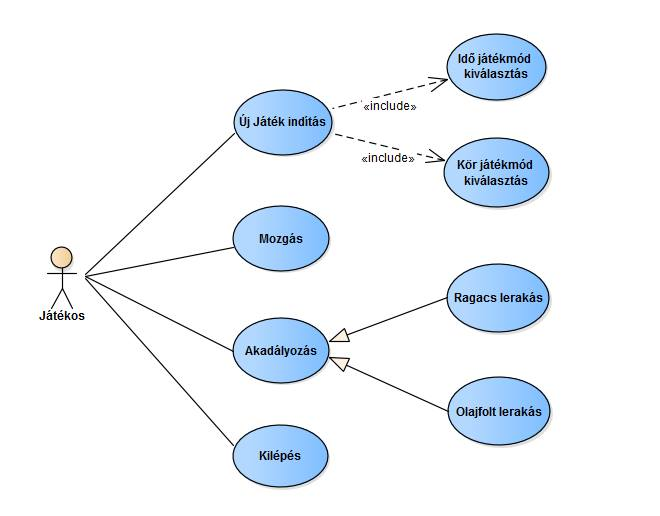
\includegraphics[scale=0.6]{use-case.jpg}
\caption{Use-Case diagram}
\label{fig:my_label}
\end{figure}


\section{Szótár}
\begin{itemize}
\item \textbf{Játékos} - A program felhasználója, a robot irányítója, aki játszik.
\item \textbf{Robot} - A játékos által irányított virtuális gépezet. Képes ugrani, ragacsot és olajat helyezni a pályára, illetve le tud esni a pályáról.
\item \textbf{Verseny} – A játék folyamata. Célja minél több kör megtétele adott idő alatt vagy adott körszám megtétele minél rövidebb idő alatt.
\item \textbf{Pálya} - A verseny helyszíne: az a sík, amin a játék zajlik. A játék közben nem változik, a robotok ide helyezhetik az olajfoltokat és a ragacsokat.
\item \textbf{Start} – Az az időpillanat, amikor a játék elindul és a játékosok megkezdik a versenyzést. Ezt egy visszaszámlálás előzi meg.
\item \textbf{Checkpoint} – Olyan vonal a pályán, ami ellenőrzi, hogy a játékos megfelelő irányban halad és nem próbál szabálytalanságot elkövetni.
\item \textbf{Célvonal} – Ha játékosok adott körszám megtételéig versenyeznek, akkor az a Checkpoint, amit bizonyos körszám után elérve a játéknak vége van.
\item \textbf{Startvonal} – Az a Checkpoint, amiről a robotok elindulnak.
\item \textbf{Idő lejárta} – Az a pillanat, amikor a játékosok rendelkezésére álló idő elfogy, eléri a nullát. Ilyenkor az adott játéknak vége van.
\item \textbf{Kör} - Egy vonal a pályán, ami minden Checkpointot pontosan egyszer érint és a kezdő- és végpontja a startvonal.
\item \textbf{Távolság} – Az a mértékegység, ami megmondja, hogy egy robot milyen hosszú utat tett meg a pályán a verseny ideje alatt.
\item \textbf{Zászlók} – Az az indikátor, ami jelzi, hogy a játékos éppen hány Checkpointon jutott át az adott körben. Minden kör végén törlődik, de a megtett körök száma megnő eggyel.
\item \textbf{Akadály} - Olyan objektum a pályán, ami megnehezíti a játékosok célba jutását. Lehet állandó, ami megmarad a játék egész ideje alatt, illetve ideiglenes, ami eltűnik, amint egy robot ráugrik.
\item \textbf{Lyuk} – Állandó akadály, amit a pálya előre tartalmaz, tehát nem a játékosok helyezik el. Ha egy robot ráugrik, akkor tönkre teszi annak felépítését, ezáltal megakadályozza a verseny folytatásában.
\item \textbf{Felszerelés} – Ragacs vagy olaj, amit a robot magánál hord és bármelyik lépésnél a pályára helyezhet. Lehelyezése után ideiglenes akadályként funkcionál.
\item \textbf{Ragacs} – Olyan ideiglenes akadály, ami felezi a ráugró robot sebességének a nagyságát.
\item \textbf{Olaj} – Olyan ideiglenes akadály, ami megakadályozza a ráugró robot irányának megváltoztatását.
\item \textbf{Irányítás} – Az a folyamat, amikor a játékos a hozzá tartozó robot irányát megváltoztatja.
\item \textbf{Irány} – A robot sebességének az a komponense, ami meghatározza, hogy a robot hova fog érkezni egy ugrás után.
\item \textbf{Sebesség} – Egy kétdimenziós vektor a pálya síkjában, ami eredendően egységnyi méretű minden robotra. Méretét csak ragacsok tudják változtatni. Irányát a játékosok irányítása, illetve az ütközések módosítják.
\item \textbf{Ugrás} – A robotok helyváltoztatási folyamata a pályán. Az ugrás nagyságát a robothoz tartozó sebességvektor nagysága határozza meg.
\item \textbf{Leesés} – Az az esemény, amikor egy robot a pálya felületén kívülre ugrik, ezáltal elhagyva a pályát.  
\item \textbf{Ütközés} – Az az esemény, amikor a két robot egymásra ugrik, azaz minimum érintik egymást egy ugrás után. A következő ugrás irányát ilyenkor a játékos nem változtathatja, hanem az az ütközésnek megfelelően módosul.
\item \textbf{Diszkvalifikáció} - A pálya elhagyásának, a pályáról való leesésnek a következménye. Ilyenkor a pályát elhagyó robotot irányító játékos veszít.
\item \textbf{Szabálytalanság} – Az az eset, amikor a játékos nem az előírt sorrendben próbál végighaladni a Checkpointokon.

\end{itemize}


\section{Projekt terv}
\subsection{Csapat}
A csapat 5 főből áll. A következő táblázat a személyes preferenciákat tartalmazza, a feladatokat úgy osztjuk ki, hogy közel azonos nehézségűek legyenek, miközben ezeket a preferenciákat szem előtt tartjuk.


\begin{longtable}{| l | l |}
\hline
\textbf{Név}   & \textbf{Felelősségek}  \tabularnewline
\hline
\hline Kovács Levente Ákos & UML, kód  \tabularnewline
\hline Lovász Attila Bence & UML, kód  \tabularnewline
\hline Graics Vince & Dokumentáció, kód  \tabularnewline
\hline Magyar Milán Bertalan & Grafika, Dokumentáció, kód  \tabularnewline
\hline Tóth Krisztián Dávid (csapatvezető) & Menedzsment, Dokumentáció, kód  \tabularnewline
\hline
\end{longtable}

\subsection {Kommunikáció}

\textbf{GitWiki}

\textbf{Elérhetőség}

\textbf{Levelezőlista}

\textbf{Megbeszélések}


\subsection{Használt programok}

\textbf{Verziókezelés}

\textbf{Dokumentáció}

\textbf{Fejlesztőkörnyezet}


\subsection{Mérföldkövek, határidők}


\begin{longtable}{| l | l | l | l | l | l |}
\hline
\textbf{Dátum}   & \textbf{Leírás} & \textbf{Ellenőrzés} \tabularnewline
\hline
\hline 2015.02.23 & Követelmény, projekt, funkcionalitás & beadás  \tabularnewline
\hline 2015.03.02 & Analízis modell kidolgozása 1. & beadás  \tabularnewline
\hline 2015.03.09 & Analízis modell kidolgozása 2. & beadás  \tabularnewline
\hline 2015.03.16 & Szkeleton tervezése & beadás  \tabularnewline
\hline 2015.03.23 & Szkeleton & beadás  \tabularnewline
\hline 2015.03.25 & \textbf{Szkeleton} & bemutatás  \tabularnewline
\hline 2015.03.30 & Prototípus koncepciója & beadás  \tabularnewline
\hline 2015.04.07 & Részletes tervek & beadás  \tabularnewline
\hline 2015.04.20 & Prototípus & beadás  \tabularnewline
\hline 2015.04.22 & \textbf{Prototípus} & bemutatás  \tabularnewline
\hline 2015.04.27 & Grafikus felület specifikációja & beadás  \tabularnewline
\hline 2015.05.11 & Grafikus változat & beadás  \tabularnewline
\hline 2015.05.13 & \textbf{Grafikus változat} & bemutatás  \tabularnewline
\hline 2015.05.15 & Összefoglalás & beadás  \tabularnewline
\hline
\end{longtable}


\textbf{szkeleton}

\textbf{prototípus}

\textbf{grafikus}


